% Asset ID: AS2StatisticalDistributionsTikZ-001
% Source: Chapter 6 Statistical Distributions transcript, discrete uniform distribution section
% Related lesson section: Key Definitions and Notation
% Purpose: Show a fair die as a discrete uniform distribution.

\documentclass[tikz,border=8pt]{standalone}
\usepackage{amsmath}
\usetikzlibrary{arrows.meta}

\begin{document}
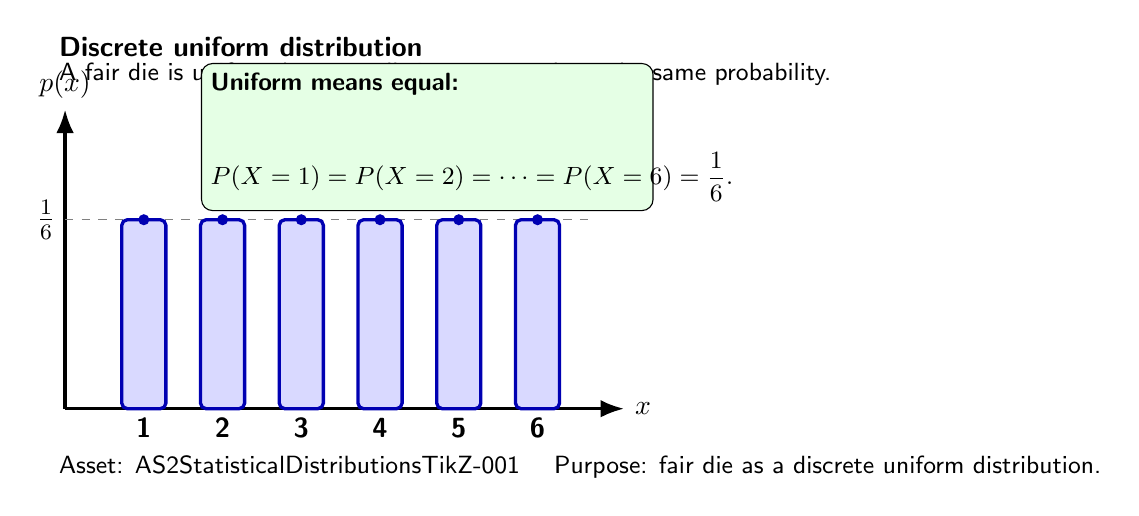
\begin{tikzpicture}[axis/.style={very thick, -{Latex[length=3mm]}},bar/.style={draw=blue!70!black, fill=blue!15, very thick, rounded corners=2pt},label/.style={font=\sffamily\bfseries},note/.style={font=\sffamily\small},mathnote/.style={font=\large}]
\node[anchor=west, label] at (-0.2,4.6) {Discrete uniform distribution};
\node[anchor=west, note] at (-0.2,4.25) {A fair die is uniform because all six outcomes have the same probability.};
\draw[axis] (0,0) -- (7.1,0) node[right, label] {$x$};
\draw[axis] (0,0) -- (0,3.8) node[above, label] {$p(x)$};
\draw[dashed, gray] (0,2.4) -- (6.7,2.4);
\node[left, mathnote] at (0,2.4) {$\frac16$};
\foreach \x in {1,2,3,4,5,6} {\draw[bar] (\x-0.28,0) rectangle (\x+0.28,2.4);\fill[blue!70!black] (\x,2.4) circle (2pt);\node[below, label] at (\x,0) {\x};}
\node[draw=black,fill=green!10,rounded corners,align=left,text width=5.5cm,note] at (4.6,3.45){\textbf{Uniform means equal:}\\[2pt] \[P(X=1)=P(X=2)=\cdots=P(X=6)=\frac16.\]};
\node[anchor=west, note] at (-0.2,-0.75) {Asset: AS2StatisticalDistributionsTikZ-001 \quad Purpose: fair die as a discrete uniform distribution.};
\end{tikzpicture}
\end{document}
